\documentclass[a4paper]{article}

\usepackage[spanish]{babel}
	\selectlanguage{spanish}
\usepackage{geometry}
	\newgeometry{margin=3cm}
\usepackage{setspace}
\usepackage{graphicx}
\usepackage{float}
\usepackage[utf8]{inputenc}

\title{Reporte del Producto 5}
\author{Ana Gabriela Carretas Talamante}
\date{17 de marzo de 2015}

\begin{document}
\maketitle
\section{Tiro Parabólico}
Se denomina movimiento parabólico al realizado por un objeto cuya trayectoria describe una parábola. Se corresponde con la trayectoria ideal de un proyectil que se mueve en un medio que no ofrece resistencia al avance y que está sujeto a un campo gravitatorio uniforme. Puede ser analizado como la composición de dos movimientos rectilíneos: un movimiento rectilíneo uniforme horizontal y un movimiento rectilíneo uniformemente acelerado vertical. 
\begin{figure}[H]
    \centering
    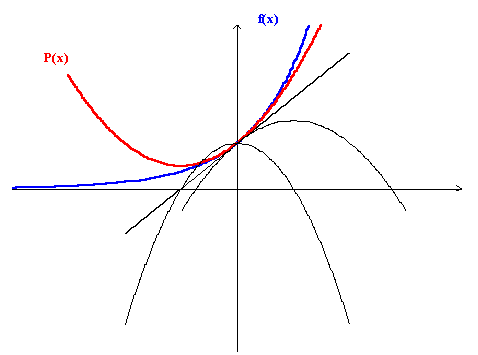
\includegraphics[width=12cm]{1}
  \end{figure} 
  
\subsection{Ecuaciones de tiro parabólico}
\label{uno}

Para cualquier instante del movimiento, la posición del proyectil tiene dos componentes $(x,y)$. La velocidad también tiene las dos coordenadas $(V_x$ y $V_y)$, estas componentes se calculan de la siguiente manera:
\begin{equation} 
\label{1}
V_ox=V_ocos\theta
\end{equation}
\label{2}
\begin{equation}
V_oy=V_osen\theta
\end{equation}

Verticalmente el movimiento es uniformemente acelerado. La única fuerza que actúa sobre el proyectil es la gravedad, por lo que la aceleración es $g$. Para cualquier instante del movimiento la velocidad vertical $(V_y)$ debe calcularse como si fuera lanzamiento vertical. Se utilizan las siguientes ecuaciones:
\begin{equation}
\label{3}
V_o=V_osen\theta-gh
\end{equation}
\begin{equation}
\label{4}
y=y_o+V_ot-\frac{gt^2}{2}
\end{equation}
\begin{equation}
\label{5}
V_y^2=(V_osen\theta)^2-2gy
\end{equation}

Horizontalmente la velocidad es constante $V_x=V_ocos\theta$ y debe calcularse como si fuera movimiento rectilíneo uniforme:
\begin{equation}
\label{6}
V_x=V_ocos\theta t
\end{equation}

\section{Simulando un tiro parabólico}
  \subsection{Código}

    Para determinar de forma unívoca la trayectoria de un proyectil, solo es necesario conocer 2 cantidades: la rapidez inicial $v$ y el ángulo $\theta$ con el que se lanzó.\\

Se proporcionó el siguiente código en \texttt{Fortran}, créditos a Waleed Ishak, para calcular la trayectoria del proyectil:
    
    \subparagraph{Código en \texttt{Fortran}}
      \begin{verbatim}
!************************************************  
!This program plots projectile motion of an object.  
!The program requires user input for initial velocity   
!and angle of the object.The algorithm uses a time   
!step of 0.01 second i.e. it calculates object's  
!location in the x and y plane every 0.01 second.  
!**********By: Waleed Ishaque, 2013**************  
program projectile_plot  
  implicit none  
  !Defining constants:  
  real, parameter :: pi = 4.0*atan(1.0) 
  real :: u, a, t, a_grados  
  real, parameter :: g = 9.81  
  real:: x(150),y(150)  
  integer :: i 

  !where g is gravity, pi is "pi"   
  !u is object's initial velocity   
  !a is object's initial angle   
  !t is time during the simulation   
  !x and y are arrays with 150 rows   
  !Seek user input   
  write(*,*) 'Enter angle of projectile (Real)'   
  read *, a_grados   
  write(*,*) 'Enter velocity of projectile (Real)'   
  read *, u   
  !Convert angle to radians   
  a = a_grados*pi/180.0   
  !open .dat file and start writing on it using the algorithm   
  open(1, file='proj.dat')   
 
  do i=1,100   
    !displacement of object in x and y direction   
    t = (float(i)*0.01)   
    x(i) = u*cos(a)*t   
    y(i) = u*sin(a)*t - 0.5*g*t*t   
    !write output in file "proj.dat" for plotting   
    write(1,*) x(i), y(i)   
    !kill the loop when the object hits the ground   
    if (y(i)<0) exit   
  end do   
  close(1)   
  !close file   
end program projectile_plot 
      \end{verbatim}
      
Este código se vio modificado, agregándole el cálculo del tiempo total de vuelo, la altura máxima que alcanza, y el alcance máximo del proyectil. Se utilizaron las ecuaciones mencionadas en la sección \ref{uno}.

\subparagraph{Código modificado en \texttt{Fortran}}
\begin{verbatim}
!************************************************  
!This program plots projectile motion of an object.  
!The program requires user input for initial velocity   
!and angle of the object.The algorithm uses a time   
!step of 0.01 second i.e. it calculates object's  
!location in the x and y plane every 0.01 second.  
!**********By: Waleed Ishaque, 2013************** 

!Modificaciones para el curso de Programacion en FORTRAN
!Universidad de Sonora, Gabriela Carretas, 2015.
program proyectil 
     implicit none  
     !Definimos las constantes:
     real, parameter :: pi = 4.0*atan(1.0) 
     real :: vo, ag, ar, t, h, r, vx, vy  
     real, parameter :: g = 9.80  
     real:: x(1000),y(1000)  
     integer :: i 

     !g es la gravedad, pi es "pi"
     !vo es la velocidad inicial del objeto   
     !ag es el angulo inicial del objeto 
     !ar es el angulo inicial del objeto convertido a radianes  
     !t es el tiempo total de vuelo
     !r es la distancia maxima de x
     !h es la altura maxima que alcanza el proyectil
     !x,y son las componentes de velocidad respectivas
     !i es un contador de desplazamiento

     !El usuario debe proporcionar datos iniciales  
     write(*,*) 'Ingrese el angulo del proyectil (Real)'   
     read *, ag   
     write(*,*) 'Ingrese la velocidad del proyectil (Real)'   
     read *, vo   
     
     !Para convertir el angulo a radianes   
     ar = ag*pi/180.0
     
     !Las componentes de velocidades
     vx = vo*cos(ar)
     vy = vo*sin(ar)

     !Comenzaremos a graficar con este algoritmo   
     open(1, file='proyectil.dat')   
     do i=1,1000
        !Calculamos las componentes de velocidad en x,y cada decima de segundo  
        t = (float(i)*0.01)   
        x(i) = vx*t   
        y(i) = vy*t - 0.5*g*t*t   
        !Escribimos los resultados en el algoritmo graficador   
        write(1,*) x(i), y(i)  
        !El programa termina cuando vuelve al suelo   
        if (y(i)<0) exit   
     end do
     close(1)
     
     !Calculamos el tiempo total de vuelo
     t = (2*vy)/g

     !Calculamos la altura maxima del proyectil
     h = (vy*vy)/2*g 

     !Calculamos la distancia maxima condicionada
     IF (ag<=0) THEN
        r = 0
     ELSE IF (ag==90) THEN
        r = 0
     ELSE
        r = vx*t
     ENDIF

     !Generamos los resultados para el usuario
     write (*,*) 'Para un proyectil con velocidad inicial=',vo,'m/s y un angulo=',ag,'grados'
     write (*,*) 'Resultados:'
     write (*,*) 'Tiempo total de vuelo=',t,'s'
     write (*,*) 'Altura maxima=',h,'m'
     write (*,*) 'Distancia maxima=',r,'m'

     !cerramos el programa   
end program proyectil 
\end{verbatim}

Ahora, hacemos énfasis en el código que se encarga de guardar los datos arrojados por el programa cada centésima de segundo, en 1000 ocasiones. Este se encarga de crear un archivo \texttt{.dat} con el cual próximamente graficaremos en el programa \texttt{gnuplot} desde la terminal.

\begin{verbatim}
     !Comenzaremos a graficar con este algoritmo   
     open(1, file='proyectil.dat')   
     do i=1,1000
        !Calculamos las componentes de velocidad en x,y cada decima de segundo  
        t = (float(i)*0.01)   
        x(i) = vx*t   
        y(i) = vy*t - 0.5*g*t*t   
        !Escribimos los resultados en el algoritmo graficador   
        write(1,*) x(i), y(i)  
        !El programa termina cuando vuelve al suelo   
        if (y(i)<0) exit   
     end do
     close(1)
\end{verbatim}  

Ahora se muestra el código utilizado en \texttt{gnuplot} desde la terminal para poder graficar en las diferentes ocasiones de ángulo que se ingresaron. \\
\begin{verbatim}set title "Tiro con angulo de -- grados y vo= -- m/s" 
set xlabel "Distancia"
set ylabel "Altura (Escala = 1/10)"
set grid
plot "proyectil.dat"
\end{verbatim}

\subsection{Corriendo el programa}
\label{dos}

\subsubsection{Ángulo de 0 grados}
\begin{figure}[H]
    \centering
    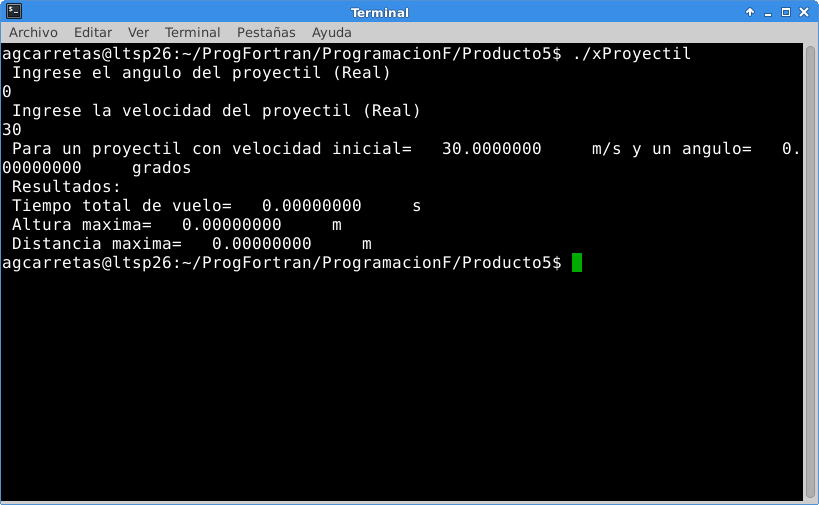
\includegraphics[width=12cm]{0} \\
    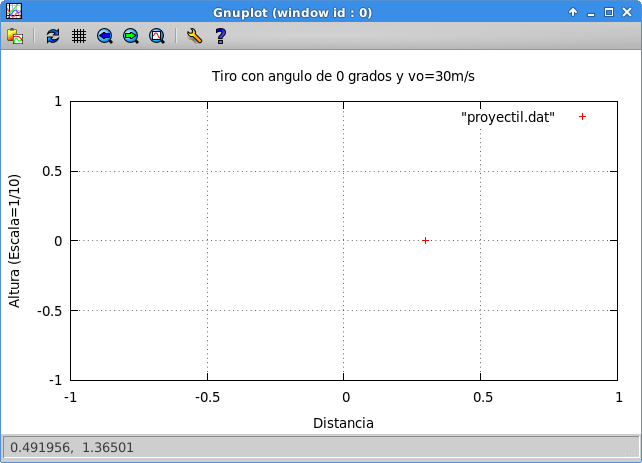
\includegraphics[width=12cm]{0plot}
  \end{figure} 

\subsubsection{Ángulo de 30 grados}
\begin{figure}[H]
    \centering
    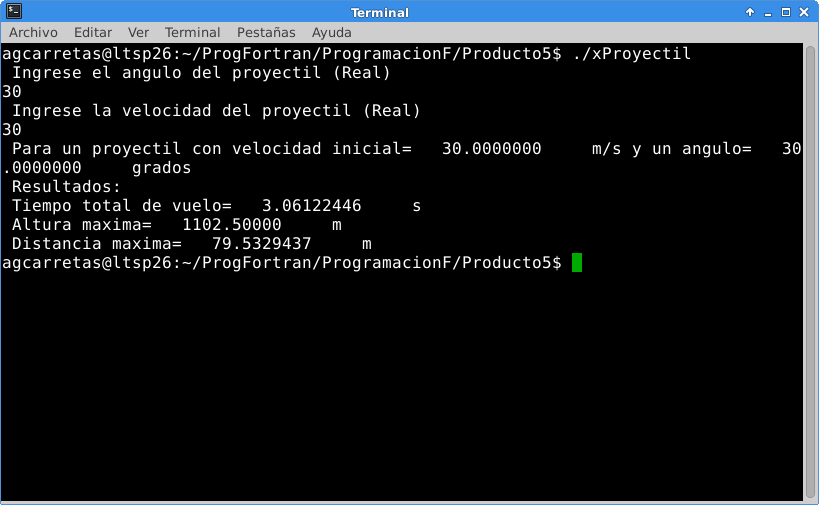
\includegraphics[width=12cm]{30} \\
    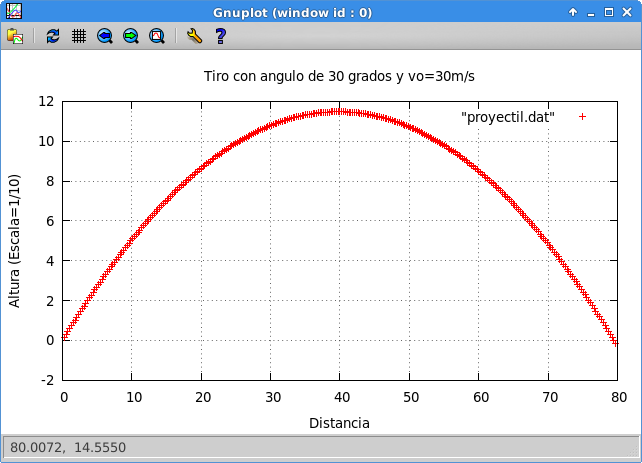
\includegraphics[width=12cm]{30plot}
  \end{figure} 

\subsubsection{Ángulo de 60 grados}
\begin{figure}[H]
    \centering
    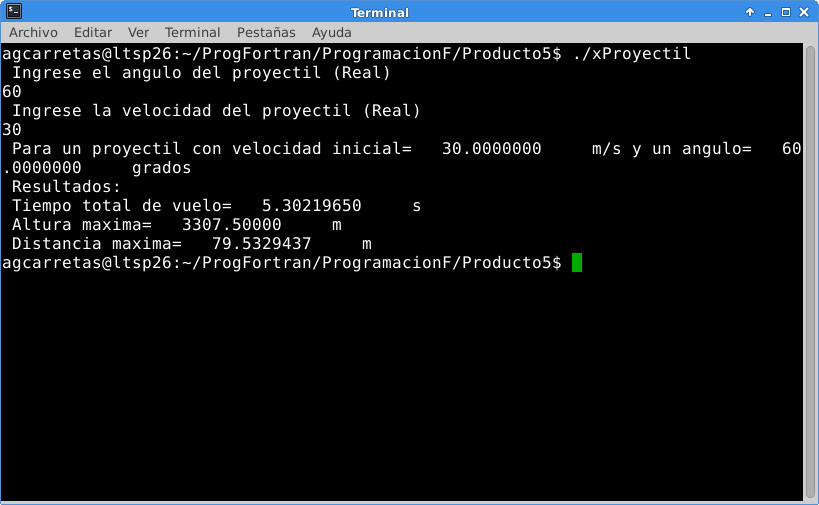
\includegraphics[width=12cm]{60} \\
    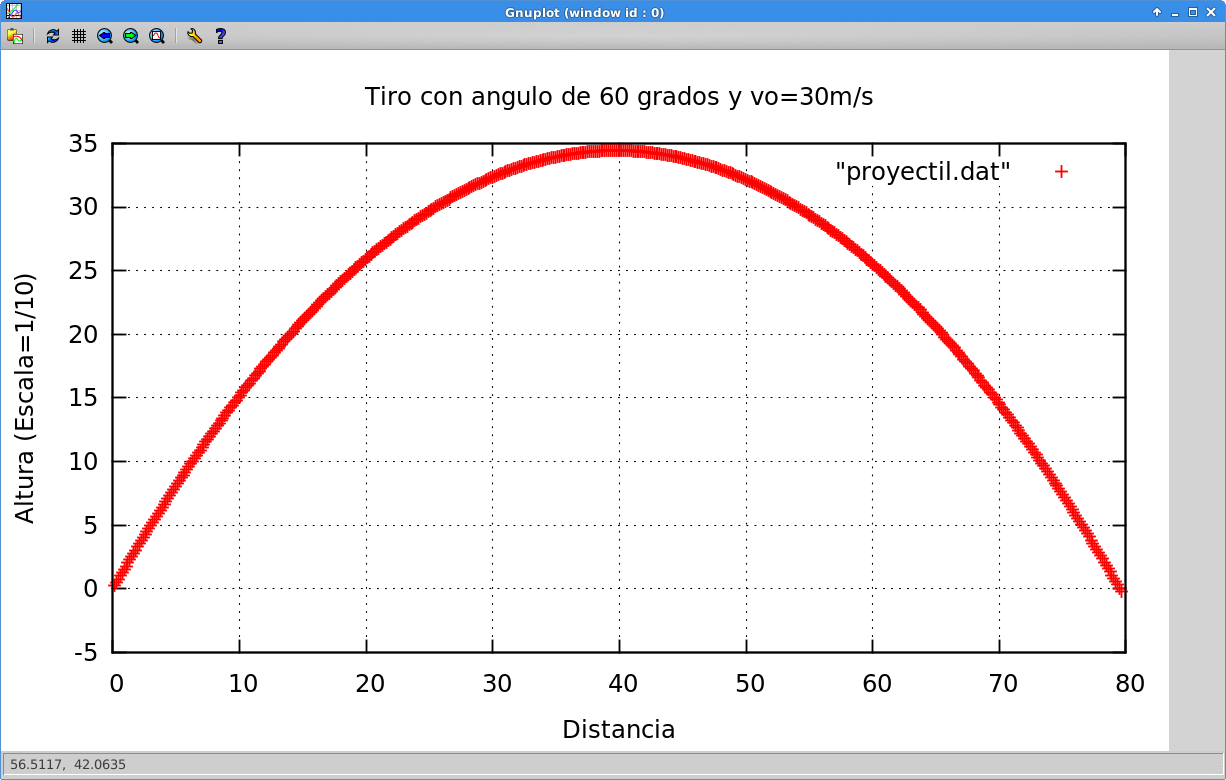
\includegraphics[width=12cm]{60plot}
  \end{figure} 

\subsubsection{Ángulo de 90 grados}
\begin{figure}[H]
    \centering
    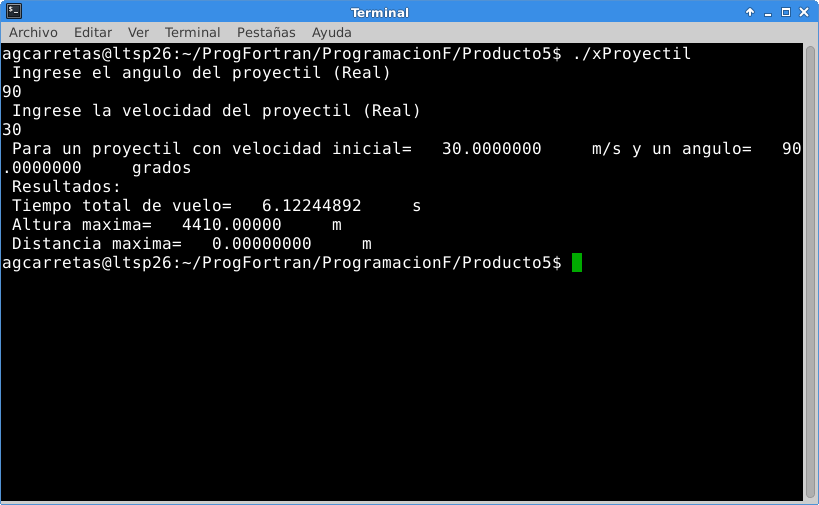
\includegraphics[width=12cm]{90} \\
    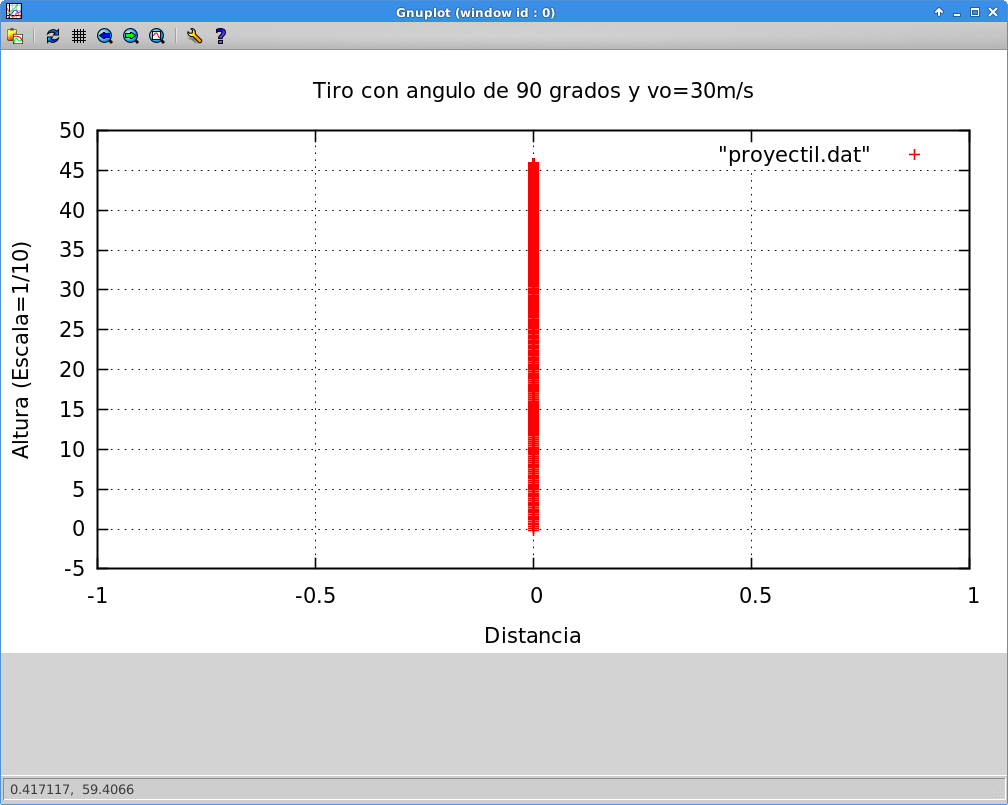
\includegraphics[width=12cm]{90plot}
  \end{figure} 

\end{document}
